%% Copernicus Publications Manuscript Preparation Template for LaTeX Submissions
%% ---------------------------------
%% This template should be used for the following class files: copernicus.cls, copernicus2.cls, copernicus_discussions.cls
%% The class files, the Copernicus LaTeX Manual with detailed explanations regarding the comments
%% and some style files are bundled in the Copernicus Latex Package which can be downloaded from the different journal webpages.
%% For further assistance please contact the Publication Production Office (production@copernicus.org).
%% http://publications.copernicus.org


%% Differing commands regarding the specific class files are highlighted.


%% copernicus.cls
\documentclass[gmd]{copernicus}

\begin{document}

\linenumbers

\title{MicroHH 1.0}


\author[1]{Chiel C. van Heerwaarden}
\author[1]{Bart J. H. van Stratum}
\author[2]{Thijs Heus}
\author[3]{Jeremy Gibbs}
\author[3]{Evgeni Fedorovich}

\affil[1]{Max Planck Institute for Meteorology, Hamburg, Germany}
\affil[2]{Cleveland State University, Cleveland, OH, USA}
\affil[3]{Oklahoma University, Norman, OK, USA}

%% The [] brackets identify the author to the corresponding affiliation, 1, 2, 3, etc. should be inserted.



\runningtitle{MicroHH 1.0}

\runningauthor{van Heerwaarden et al.}

\correspondence{Chiel van Heerwaarden\\ (chiel.vanheerwaarden@mpimet.mpg.de)}



\received{}
\pubdiscuss{} %% only important for two-stage journals
\revised{}
\accepted{}
\published{}

%% These dates will be inserted by the Publication Production Office during the typesetting process.


\firstpage{1}

\maketitle  %% Please note that for the copernicus2.cls this command needs to be inserted after \abstract{TEXT}

\begin{abstract}
This paper describes MicroHH 1.0, a new Computational Fluid Dynamical code for the simulation of wall-bounded turbulent flows in the atmosphere using Direct Numerical Simulation and Large-Eddy Simulation. The paper covers the description of the governing equations, their numerical implementation and the parametrizations involved in the code. Furthermore, the paper presents the validation of the dynamical core in the form of convergence tests and conservation tests and comparison of simulations of channel flows and slope flows against well-established models. The full numerical model, including the associated parametrizations for Large-Eddy simulations of high Reynolds number flows, has been tested for a set of cases under stable and unstable conditions, under the Boussinesq and anelastic approximation and with dry and moist convection under stationary and time-varying boundary conditions. The paper also presents scaling tests showing good scaling from 256 to 32,738 processes.
\end{abstract}

\introduction  %% \introduction[modified heading if necessary]
In this paper we present a description of MicroHH 1.0, a new Computational Fluid Dynamical code for the simulation of wall-bounded turbulent flows, with a focus on those in the atmosphere. MicroHH is a model that can be run both for Direct Numerical Simulations as well as for Large-Eddy Simulations with applications ranging from channel flows to cloudy boundary layers. The model has been designed and written from scratch with the aim of creating a highly parallel code that is able to run on more than 10,000 processes with the support of modern techniques. MicroHH has been written in C++, in contrast to the majority of its peers, which are written in Fortran 90 for reasons that we explain in Section \ref{sec:technical}.

In this paper we provide a full description of the governing equations and their numerical implementation. In addition, we discuss the added parametrizations and their underlying assumptions.

\section{Dynamical core: governing equations}
The dynamical core of MicroHH follows the conservation equations under the anelastic approximation as shown in BANNON1996. This approximation has the advantage that it directly simplifies to the Boussinesq equations if the base density $\rho_0$ is assumed to be constant in space.

\subsection{Conservation of mass}
\begin{eqnarray}
\dfrac{\partial \rho_0 u_i}{\partial x_i} & = & 0\label{eq:consmassa}
\end{eqnarray}

\begin{eqnarray}
\dfrac{\partial u_i}{\partial x_i} & = & 0\label{eq:consmassb}
\end{eqnarray}

\subsection{Conservation of momentum}
The momentum equation is written it the flux form, in order to assure the best possible mass and momentum conservation. The hydrostatic balance $dp_0 / dz~=~-\rho_0 g$ has been subtracted to arrive at the perturbation form:
\begin{eqnarray}
\dfrac{\partial u_i}{\partial t} & = & - \dfrac{1}{\rho_0} \dfrac{\partial \rho_0 u_i u_j}{\partial x_j} 
- \dfrac{\partial}{\partial x_i}\left(\dfrac{p'}{\rho_0}\right) + g \dfrac{\theta_v'}{\theta_{v0}} + \nu \dfrac{\partial^2 u_i}{\partial x_j^2}\label{eq:consmoma},\\
\dfrac{\theta_v'}{\theta_{v0}} & = & \dfrac{p'}{\rho g H_{\rho}} - \dfrac{\rho'}{\rho_0}\label{eq:statea},
\end{eqnarray}
where the scale height of density is defined as: $H_{\rho}~\equiv~\left( \dfrac{1}{\rho_0} \dfrac{d\rho_0}{dz} \right)^{-1}$. Under the Boussinesq approximation, where $\rho_0$ is constant with height and the scale height for density $H_\rho$ approaches infinity, the set simplifies to:
\begin{eqnarray}
\dfrac{\partial u_i}{\partial t} & = & - \dfrac{\partial u_i u_j}{\partial x_j}
- \dfrac{1}{\rho_0}\dfrac{\partial p}{\partial x_i} + g \dfrac{\theta_v'}{\theta_{v0}} + \nu \dfrac{\partial^2 u_i}{\partial x_j^2}\label{eq:consmomb},\\
\dfrac{\theta_v'}{\theta_{v0}} & = & - \dfrac{\rho'}{\rho_0}\label{eq:stateb}.
\end{eqnarray}

\subsection{Pressure equation}
For simplicity we define function $f$ that contains all right hand side terms of Eq., except the pressure gradient. In order to arrive at the equation that allows us to solve for the pressure we multiply the equation with the base density $\rho_0$ and take the divergence. Conservation of mass ensures that the tendency term vanishes, such that an elliptic equation remains for the pressure:
\begin{eqnarray}
\dfrac{\partial}{\partial x_i} 
\left[ \rho_0 \dfrac{\partial}{\partial x_i} \left( \dfrac{p'}{\rho_0} \right) \right] & = &
\dfrac{\partial \rho_0 f_i}{\partial x_i}.
\end{eqnarray}
Under the Boussinesq approximation the equation simplifies to:
\begin{eqnarray}
\dfrac{\partial^2}{\partial x_i^2} \left( \dfrac{p'}{\rho_0} \right) & = &
\dfrac{\partial f_i}{\partial x_i}.
\end{eqnarray}


\subsection{Conservation of an arbitrary scalar}
The conservation equation of an arbitrary scalar $\phi$ can be written in flux form:
\begin{eqnarray}
\dfrac{\partial \phi}{\partial t} & = & - \dfrac{1}{\rho_0} \dfrac{\partial \rho_0 u_j \phi}{\partial x_j} +
\kappa_\phi \dfrac{\partial^2 \phi}{\partial x_j^2} + S_\phi,
\end{eqnarray}
where $S_\phi$ represents sources and sinks of the variable.

\subsection{Conservation of energy}
MicroHH supports a series of governing equations for the energy equation. In short there are two modes, one that uses the potential temperature as a prognostic variable
\begin{eqnarray}
\dfrac{\partial \theta}{\partial t} & = & - \dfrac{1}{\rho_0} \dfrac{\partial \rho_0 u_j \theta}{\partial x_j} + \kappa_\phi \dfrac{\partial^2 \theta}{\partial x_j^2} + \dfrac{\theta_0}{\rho_0 c_p T_0} Q,
\end{eqnarray}
and one that uses the liquid water potential temperature $\theta_l$.



\subsection{Simplification of the Boussinesq system and the extension to slope flows}
Under the Boussinesq approximation with only dry thermodynamics ($\theta_v = \theta$), the equation of state can be eliminated and the conservation of momentum and energy can be written as:
\begin{eqnarray}
\dfrac{\partial u_i}{\partial t} + \dfrac{\partial u_i u_j}{\partial x_j} & = & 
- \dfrac{1}{\rho_0}\dfrac{\partial p'}{\partial x_i} + \delta_{i3} b + \nu \dfrac{\partial^2 u_i}{\partial x_j^2}\label{eq:consmombsimp},\\
\dfrac{\partial b}{\partial t} + \dfrac{\partial b u_j}{\partial x_j} & = & 
\kappa_b \dfrac{\partial^2 b}{\partial x_j^2}\label{eq:consenbsimp}
\end{eqnarray}

With a slight modification to the previous set of equations, it is possible to study slope flows in periodic domains. If we no longer assume that gravity is directed along the z-axis, but instead assume that the domain is under a slope $\alpha$ such that gravity is distributed between the x-axis and z-axis, and assume that the reference buoyancy increases with height with slope $N^2$, the equations can be written as:
\begin{eqnarray}
\dfrac{\partial u}{\partial t} + \dfrac{\partial u_j u}{\partial x_j} & = & 
- \dfrac{1}{\rho_0}\dfrac{\partial p'}{\partial x} + sin(\alpha) b + \nu \dfrac{\partial^2 u}{\partial x_j^2}\label{eq:consuslope},\\
\dfrac{\partial w}{\partial t} + \dfrac{\partial u_j w}{\partial x_j} & = & 
- \dfrac{1}{\rho_0}\dfrac{\partial p'}{\partial z} + cos(\alpha) b + \nu \dfrac{\partial^2 w}{\partial x_j^2}\label{eq:conswslope},\\
\dfrac{\partial b}{\partial t} + \dfrac{\partial b u_j}{\partial x_j} & = & 
\kappa_b \dfrac{\partial^2 b}{\partial x_j^2} - \left (u\,sin(\alpha) + w\,cos(\alpha) \right) N^2\label{eq:consbslope}
\end{eqnarray}


\section{Dynamical core: numerical implementation}
\subsection{Time integration}
The prognostic equations are solved using low-storage Runge-Kutta time integration schemes, where each prognostic variable requires only two three dimensional fields. The code provides two options: a three-stage third order scheme (WILSON) and a five stage fourth order scheme (CARPENTER). Both of them can be written in the same general form in semi-discrete formulation:
\begin{eqnarray}
f\left(\phi^n\right) & = & a^n f\left( \phi^{n-1} \right) \\
\phi^{n+1} & = & \phi^n + b^n \Delta t f\left(\phi^n\right),
\end{eqnarray}
where $f$ is a function that represent the computation of all right hand side terms, $\phi$ is an arbitrary variable and $a$ and $b$ are the coefficients for the Runge-Kutta method at stage $n$. In principle, in low storage form, the tendencies of the previous stage $n-1$ are retained and multiplied with $a^n$ at the beginning of a stage, except for the first stage, where $a_1 = 0$. During the time integration, the tendency is multiplied with coefficient $b^n$ in order to find the value of arbitrary variable $\phi$ in stage $n+1$.

For the third-order scheme the vectors $a$ and $b$ are:
\begin{eqnarray}
a & = & \left\{0, -\frac{5}{9}, -\frac{153}{128} \right\}\\
b & = & \left\{\frac{1}{3}, \frac{15}{16}, \frac{8}{15} \right\}
\end{eqnarray}

For the fourth-order scheme the vectors $a$ and $b$ are:
\begin{eqnarray}
\nonumber a & = & \left\{0, -\frac{567301805773}{1357537059087},
-\frac{2404267990393}{2016746695238},\right.\\
& & \left. -\frac{3550918686646}{2091501179385},
-\frac{1275806237668}{842570457699} \right\}\\
\nonumber b & = & \left\{\frac{1432997174477}{9575080441755}, \frac{5161836677717}{13612068292357},
\frac{1720146321549}{2090206949498},\right.\\
& & \left. \frac{3134564353537}{4481467310338},
\frac{2277821191437}{14882151754819} \right\}
\end{eqnarray}

Even though the fourth order scheme has five stages and is thus considerably more expensive than the third order scheme, the truncation error is so much smaller that under most conditions it pays off to use fourth order scheme. We demonstrate this in Section \ref{sec:validationtime}, where we study the conservation properties of the model and the accuracy of the time integration scheme.

\subsection{Grid}
MicroHH is discretized on a staggered grid, where the scalars are located in the middle of a grid cell and the three velocity components on the boundaries. 

\subsection{Building blocks of the spatial discretization}
The spatial operators are based on finite differences. The code supports second order and fourth order accurate discretizations, which follow \citet{Morinishi1998, Vasilyev2000}. From Taylor series spatial operators can be derived that form the building blocks of more advanced operators, such as the advection and diffusion operators. In the following section we describe for simplicity the operators and the derived operators in two dimensions.

First, there are the second order accurate interpolation operators:
\begin{eqnarray}
\phi_{i,j} \approx \widehat{\phi}^{2x }_{i,j} & \equiv & \dfrac{\phi_{i-\frac{1}{2},j} + \phi_{i+\frac{1}{2},j}}{2},\\
\phi_{i,j} \approx \widehat{\phi}^{2xL}_{i,j} & \equiv & \dfrac{\phi_{i-\frac{3}{2},j} + \phi_{i+\frac{3}{2},j}}{2},
\end{eqnarray}

\begin{eqnarray}
\left. \dfrac{\partial \phi}{\partial x}\right|_{i,j} \approx \delta_{2x} \left( \phi \right)_{i,j} \equiv \dfrac{\phi_{i+\frac{1}{2},j} - \phi_{i-\frac{1}{2},j}}
                                                                                                                 {   x_{i+\frac{1}{2}}   -    x_{i-\frac{1}{2}  }}
\end{eqnarray}

\begin{eqnarray}
\left. \dfrac{\partial \phi}{\partial x}\right|_{i,j} \approx \delta_{2xL} \left( \phi \right)_{i,j} \equiv \dfrac{\phi_{i+\frac{3}{2},j} - \phi_{i-\frac{3}{2},j}}
                                                                                                                  {   x_{i+\frac{3}{2}}   -    x_{i-\frac{3}{2}  }}
\end{eqnarray}

\begin{eqnarray}
\delta_{2x} \left( \phi \right)_{i,j} = \dfrac{\phi_{i+\frac{1}{2},j} - \phi_{i-\frac{1}{2},j}}
                                              {\Delta x}
\end{eqnarray}

\begin{eqnarray}
\delta_{2xL} \left( \phi \right)_{i,j} = \dfrac{\phi_{i+\frac{3}{2},j} - \phi_{i-\frac{3}{2},j}}
                                               {3\Delta x}
\end{eqnarray}

\subsubsection{Fourth order operators}

\begin{eqnarray}
\phi_{i,j} \approx \widehat{\phi}^{4x}_{i,j} \equiv \dfrac{- \phi_{i-\frac{3}{2},j} + 9 \phi_{i-\frac{1}{2},j} + 9 \phi_{i+\frac{1}{2},j} - \phi_{i+\frac{3}{2},j}}{16}\label{eq:interp4}
\end{eqnarray}

\begin{eqnarray}
\phi_{i,j} \approx \widehat{\phi}^{4xb}_{i,j} \equiv \dfrac{ 5 \phi_{i-\frac{1}{2},j} + 15 \phi_{i+\frac{1}{2},j} - 5 \phi_{i+\frac{3}{2},j} + \phi_{i+\frac{5}{2},j}}{16}
\end{eqnarray}

\begin{eqnarray}
\nonumber
\left. \dfrac{\partial \phi}{\partial x}\right|_{i,j} & \approx & \delta_{4x} \left( \phi \right)_{i,j}\\
& \equiv & \dfrac{\phi_{i-\frac{3}{2},j} - 27 \phi_{i-\frac{1}{2},j} + 27 \phi_{i+\frac{1}{2},j} - \phi_{i+\frac{3}{2},j}}
             {       x_{i-\frac{3}{2}}   - 27    x_{i-\frac{1}{2}}   + 27    x_{i+\frac{1}{2}}   -    x_{i+\frac{3}{2}}}
\end{eqnarray}

\begin{eqnarray}
\nonumber
\left. \dfrac{\partial \phi}{\partial x}\right|_{i,j} & \approx & \delta_{4xb} \left( \phi \right)_{i,j}\\
& \equiv & \dfrac{-23 \phi_{i-\frac{1}{2},j} + 21 \phi_{i+\frac{1}{2},j} + 3 \phi_{i+\frac{3}{2},j} - \phi_{i+\frac{5}{2},j}}
                 {-23    x_{i-\frac{1}{2}}   + 21    x_{i+\frac{1}{2}}   + 3    x_{i+\frac{3}{2}}   -    x_{i+\frac{5}{2}}}
\end{eqnarray}

\begin{eqnarray}
\delta_{4x} \left( \phi \right)_{i,j}  = \dfrac{\phi_{i-\frac{3}{2},j} - 27 \phi_{i-\frac{1}{2},j} + 27 \phi_{i+\frac{1}{2},j} - \phi_{i+\frac{3}{2},j}}
                                               {24 \Delta x}
\end{eqnarray}
% \begin{eqnarray}
% \nonumber 
% &&\left. \dfrac{\partial^2 \phi}{\partial x^2}\right|_{i,j} \approx \delta_{4x} \left( \delta_{4x} \left( \phi \right) \right)_{i,j}\\
% \nonumber
% && = \dfrac{1}{576 \left( \Delta x \right)^2} \left( \phi_{i-3,j} - 54 \phi_{i-2,j} + 783 \phi_{i-1,j}\right.\\
% &&  \left. - 1460  \phi_{i,j} + 783 \phi_{i+1,j} - 54 \phi_{i+2,j} + \phi_{i+3,j} \right)
% \end{eqnarray}

\subsection{Advection}
The advection term is discretized in the flux form:
\begin{eqnarray}
\nonumber
\dfrac{\partial u \phi}{\partial x} + \dfrac{\partial v \phi}{\partial y} & \approx & \delta_{2x} \left( u \widehat{\phi}^{2x} \right)_{i,j} \\ 
& = & \dfrac{ u_{i+\frac{1}{2},j} \widehat{\phi}^{2x}_{i+\frac{1}{2},j} - u_{i-\frac{1}{2},j} \widehat{\phi}^{2x}_{i-\frac{1}{2},j} }
            { x_{i+\frac{1}{2}} - x_{i-\frac{1}{2}} }\\
& + & \dfrac{ v_{i,j+\frac{1}{2}} \widehat{\phi}^{2x}_{i,j+\frac{1}{2}} - v_{i,j-\frac{1}{2}} \widehat{\phi}^{2x}_{i,j-\frac{1}{2}} }
            { y_{j+\frac{1}{2}} - y_{j-\frac{1}{2}} }
\end{eqnarray}

\begin{eqnarray}
\dfrac{\partial v u}{\partial x} = \delta_{2x} \left( \widehat{v}^{2y} \widehat{u}^{2x} \right)_{i,j} =
\dfrac{ \widehat{v}^{2y}_{i+\frac{1}{2},j} \widehat{u}^{2x}_{i+\frac{1}{2},j} - \widehat{v}^{2y}_{i-\frac{1}{2},j} \widehat{u}^{2x}_{i-\frac{1}{2},j} }
      { x_{i+\frac{1}{2}} - x_{i-\frac{1}{2}} }\label{eq:advec2u}
\end{eqnarray}
In the standard fourth-order scheme:
\begin{eqnarray}
\nonumber
\left. \dfrac{\partial u \phi}{\partial x} \right|_{i,j} & \approx & \delta_{4x} \left( u \widehat{\phi}^{4x} \right)_{i,j} \\
\nonumber
& = & \left( u_{i-\frac{3}{2},j} \widehat{\phi}^{4x}_{i-\frac{3}{2},j} - 27 u_{i-\frac{1}{2},j} \widehat{\phi}^{4x}_{i-\frac{1}{2},j} \right.\\
\nonumber
&   &\left. + 27 u_{i+\frac{1}{2},j} \widehat{\phi}^{4x}_{i+\frac{1}{2},j} - u_{i+\frac{3}{2},j} \widehat{\phi}^{4x}_{i+\frac{3}{2},j} \right)\\
&   &\slash \left( x_{i-\frac{3}{2}} - 27 x_{i-\frac{1}{2}} + 27 x_{i+\frac{1}{2}} - x_{i+\frac{3}{2}} \right)
\end{eqnarray}
Hereafter, we assume that the usage of the operators is clear and we no longer expand them.

The fully energy conserving scheme is an interpolation of two second order operators:
\begin{eqnarray}
% \nonumber
\left. \dfrac{\partial u \phi}{\partial x} \right|_{i,j} & = & \frac{9}{8} \delta_{2x} \left( u \widehat{\phi}^{2x} \right)_{i,j} 
                                                             - \frac{1}{8} \delta_{2xL} \left( u \widehat{\phi}^{2xL} \right)_{i,j}%\\
% \nonumber
% & = & \frac{9}{16} \dfrac{ u_{i+\frac{1}{2},j} \widehat{\phi}^x_{i+\frac{1}{2},j} - u_{i-\frac{1}{2},j} \widehat{\phi}^x_{i-\frac{1}{2},j} }
%                           { x_{i+\frac{1}{2}} - x_{i-\frac{1}{2}} }\\
% & - & \frac{1}{16} \dfrac{ u_{i+\frac{3}{2},j} \widehat{\phi}^{3x}_{i+\frac{3}{2},j} - u_{i-\frac{3}{2},j} \widehat{\phi}^{3x}_{i-\frac{3}{2},j} }
%                           { x_{i+\frac{3}{2}} - x_{i-\frac{3}{2}} }
\end{eqnarray}
Note that in this scheme velocity interpolations, such as in Eq. \ref{eq:advec2u}, still need to be performed with fourth order accuracy (Eq. \ref{eq:interp4}) in order to keep the total operator fourth order accurate. Therefore, for instance:
\begin{eqnarray}
\dfrac{\partial v u}{\partial x} \approx \frac{9}{8} \delta_{2x} \left( \widehat{v}^{4y} \widehat{u}^{2x} \right)_{i,j} 
                                       - \frac{1}{8} \delta_{2xL} \left( \widehat{v}^{4y} \widehat{u}^{2xL} \right)_{i,j}
\end{eqnarray}

\subsection{Diffusion}
The diffusion operator is calculated as a divergence of a gradient:
\begin{eqnarray}
\left. \kappa_\phi \dfrac{\partial^2 \phi}{\partial x^2}\right|_{i,j} & \approx &
\kappa_\phi \delta_{2x} \left( \delta_{2x} \left( \phi \right) \right)_{i,j}\\
% \kappa_\phi \dfrac{\left. \dfrac{\partial \phi}{\partial x}\right|_{i+\frac{1}{2},j} - \left. \dfrac{\partial \phi}{\partial x}\right|_{i-\frac{1}{2},j}}
%                                 {   x_{i+\frac{1}{2},j} -    x_{i-\frac{1}{2},j}}
\left. \kappa_\phi \dfrac{\partial^2 \phi}{\partial x^2}\right|_{i,j} & \approx &
\kappa_\phi \delta_{4x} \left( \delta_{4x} \left( \phi \right) \right)_{i,j}
\end{eqnarray}
On an equidistant grid, this leads to the well-known second order accurate operator for the second derivate:
\begin{eqnarray}
\kappa_\phi \delta_{2x} \left( \delta_{2x} \left( \phi \right) \right)_{i,j} =
\kappa_\phi \dfrac{ \phi_{i-1,j} - 2 \phi_{i,j} + \phi_{i+1,j} }{\left( \Delta x \right)^2},
\end{eqnarray}
whereas for a fourth-order accurate operator, a seven-point stencil is derived:
\begin{eqnarray}
\nonumber
&& \kappa_\phi \delta_{4x} \left( \delta_{4x} \left( \phi \right) \right)_{i,j}\\
\nonumber
&& = \dfrac{\kappa_\phi}{576 \left( \Delta x \right)^2} \left( \phi_{i-3,j} - 54 \phi_{i-2,j} + 783 \phi_{i-1,j}\right.\\
&&  \left. - 1460  \phi_{i,j} + 783 \phi_{i+1,j} - 54 \phi_{i+2,j} + \phi_{i+3,j} \right)
\end{eqnarray}

% \begin{eqnarray}
% \nonumber
% \left. \kappa_\phi \dfrac{\partial^2 \phi}{\partial x^2}\right|_{i,j} & = & \kappa_\phi
% \left( \left. \dfrac{\partial \phi}{\partial x}\right|_{i-\frac{3}{2},j} 
% - 27 \left. \dfrac{\partial \phi}{\partial x}\right|_{i-\frac{1}{2},j} \right. \\
% \nonumber
% & & \left. + 27 \left. \dfrac{\partial \phi}{\partial x}\right|_{i+\frac{1}{2},j} 
% - \left. \dfrac{\partial \phi}{\partial x}\right|_{i+\frac{3}{2},j} \right)\\
% & & / \left( x_{i-\frac{3}{2}} - 27    x_{i-\frac{1}{2}} + 27    x_{i+\frac{1}{2}} -    x_{i+\frac{3}{2}} \right)
% \end{eqnarray}
\subsection{Pressure}
The pressure solver follows the method of Chorin19XX.
Modified wavenumber
\begin{eqnarray}
\left. \widetilde{u_i} \right|^{t+1}_{i,j,k} & = & \left. u_i \right|^{t}_{i,j,k} + \Delta t \left. f_i \right|^{t}_{i,j,k}\\
\left. u_i\right|^{t+1}_{i,j,k} & = & \left. \widetilde{u_i} \right|^{t+1}_{i,j,k} - \Delta t \left. \delta_{nx_i}\left( \dfrac{p}{\rho_0}\right)\right|^t_{i,j,k}
\end{eqnarray}
Bla \ref{eq:poisson}
\begin{eqnarray}
\end{eqnarray}



\subsection{Boundary conditions}
The lateral boundaries in MicroHH are periodic.

The boundary conditions can be formulated in their most general form, the Robin boundary condition:
\begin{eqnarray}
a \phi_s + b \left.\dfrac{\partial \phi}{\partial z}\right|_s = c,
\end{eqnarray}
which gives the Dirichlet boundary condition when ${a=1,~b=0}$ and the Neumann boundary condition when ${a=0,~b=1}$. 

MicroHH makes use of ghost cells in order to avoid the need of biased schemes for single interpolation or gradient operators near the wall. The values at the ghost cells are derived making use of the boundary conditions. 

The ghost cells for the Dirichlet boundary conditions in the second order accurate discretization are:
\begin{eqnarray}
\phi_{-\frac{1}{2}} & = & 2 c - \phi_{\frac{1}{2}},
\end{eqnarray}
whereas those for the Neumann boundary condition are:
\begin{eqnarray}
\phi_{-\frac{1}{2}} & = & -c \left( - z_{-\frac{1}{2}} + z_{\frac{1}{2}} \right) + \phi_{\frac{1}{2}}
\end{eqnarray}

In case of the fourth order scheme, we have two ghost cells and therefore a second boundary condition is required. Here we set the third order derivative equal to zero (see \citet{Morinishi1998}). For the Dirichlet boundary condition we arrive at the following expressions for the ghost cells:
\begin{eqnarray}
\phi_{-\frac{1}{2}} & = & \dfrac{8 c - 6 \phi_{\frac{1}{2}} + \phi_{\frac{3}{2}}}{3} \\
\phi_{-\frac{3}{2}} & = & 8 c - 6 \phi_{\frac{1}{2}} + \phi_{\frac{3}{2}},
\end{eqnarray}
whereas in case of a Neumann boundary condition we find:
\begin{eqnarray}
\phi_{-\frac{1}{2}} & = & -c  \dfrac{z_{i-\frac{3}{2}} - 27 z_{i-\frac{1}{2}} + 27 z_{i+\frac{1}{2}} - z_{i+\frac{3}{2}}}{24} + \phi_{\frac{1}{2}} \\
\phi_{-\frac{3}{2}} & = & -3c \dfrac{z_{i-\frac{3}{2}} - 27 z_{i-\frac{1}{2}} + 27 z_{i+\frac{1}{2}} - z_{i+\frac{3}{2}}}{24} + \phi_{\frac{3}{2}}
\end{eqnarray}

\section{Physical parametrizations}
\subsection{Surface model}
\subsection{Subfilter scale model}
\subsection{Thermodynamics}

\section{Technical details of the code}\label{sec:technical}
\subsection{Code structure}
MicroHH is written in C++ and makes use of aspects of object-oriented programming. Separate model components are written in classes, to allow for a straightforward substitution and to avoid unnecessary switch statements inside of the code. Public and protected functions inside of the classes are declared virtual to open the possibility of replacing them in a derived class. This organization of the code has the advantage that any extension or case-specific code can be put in its own file, in order to minime the amount of code that needs to be edited and to allow for an easier merging with newer versions of the code.

\subsection{Parallelization}
The code uses the Message Passing Interface (MPI) in order to run on a large number of processes. The code creates a Cartesian grid using the MPI\_Cart\_create function and uses this grid to detect the IDs of neighboring processes. In order to avoid complex packing routines, we make use of MPI datatypes wherever possible. The MPI calls are written in an interface, such that the typical user never has to write any MPI calls for his personal routines.

The Input/Output (IO) is entirely based on MPI-IO, such that three dimensional fields and two dimensional cross sections are stored as single files. We have chosen for MPI-IO in order to limit the number of files written by simulations done on a large number of processes and to allow for restarts on a different number of processes. In order to keep the code as clean as possible, we make use of the MPI\_Sub\_array function in combination with MPI\_File\_write\_all in order to write three dimensional fields and cross sections.

\subsection{External dependencies}
MicroHH depends on three external software tools or libraries. First, it uses the CMake build system for the generation of Makefiles. CMake allows for parallel builds, which minimizes the compilation time. Furthermore, the FFTW3 library \citep{Frigo2005} is used for the computation of the Fast-Fourier Transforms. Last, the statistical routines save their output in NetCDF format and therefore rely on UCAR's NetCDF library.

\section{Scaling experiments}
\begin{figure}[t]
\vspace*{2mm}
\begin{center}
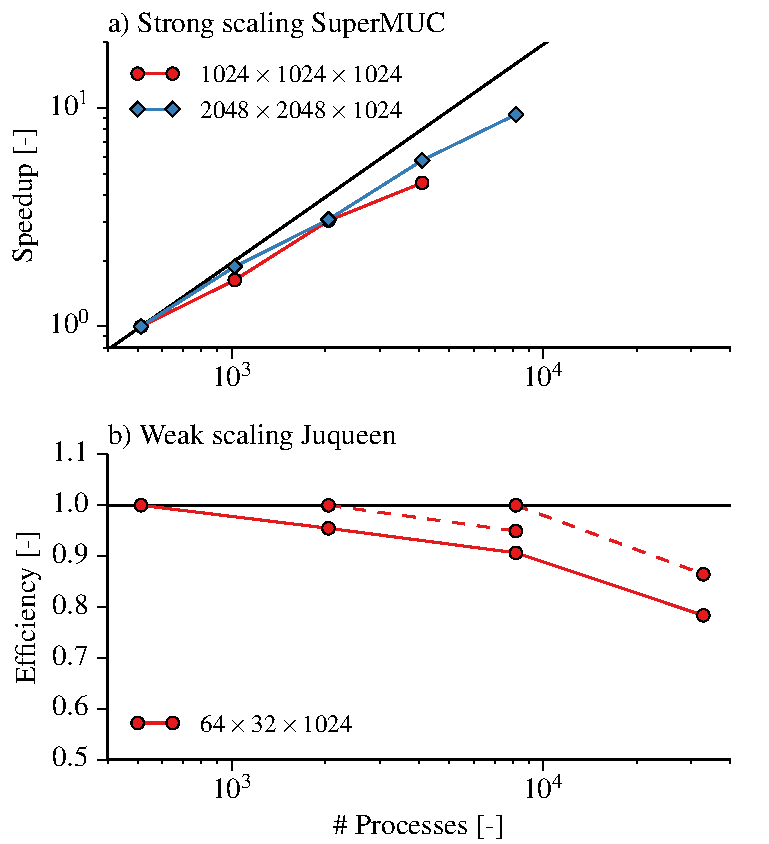
\includegraphics[width=8.3cm]{figs/scaling.pdf}
\end{center}
\caption{Error convergence of the spatial discretization in the two-dimensional Taylor-Green vortex. The dashed black line shows second-order convergence, the dotted black line shows fourth-order convergence.}
\end{figure}

\section{Model evaluation}
\subsection{Evaluation of the dynamical core}
\subsubsection{Taylor-Green vortex}
Bla.
\begin{figure}[t]
\vspace*{2mm}
\begin{center}
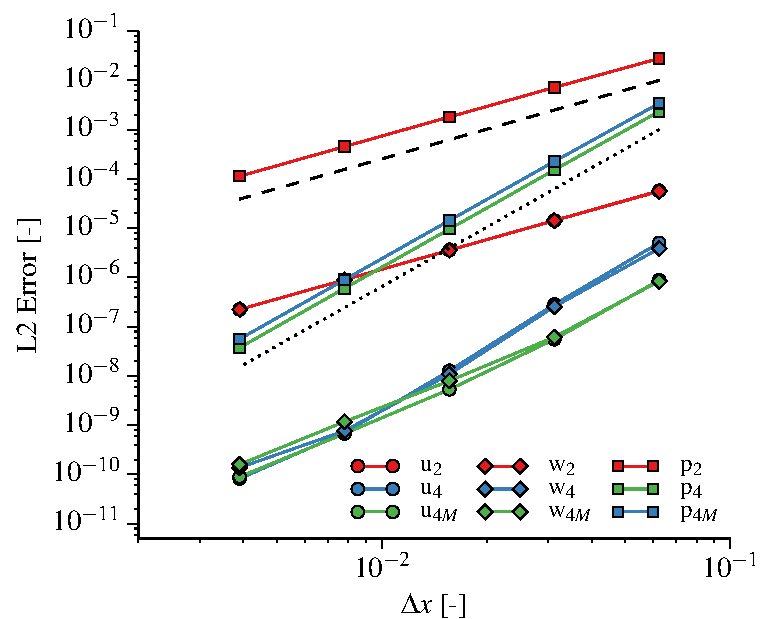
\includegraphics[width=8.3cm]{figs/taylorgreen.pdf}
\end{center}
\caption{Error convergence of the spatial discretization in the two-dimensional Taylor-Green vortex. The dashed black line shows second-order convergence, the dotted black line shows fourth-order convergence.}
\end{figure}

\subsubsection{Energy conservation and time accuracy}\label{sec:validationtime}
Bla.
\begin{figure}[t]
\vspace*{2mm}
\begin{center}
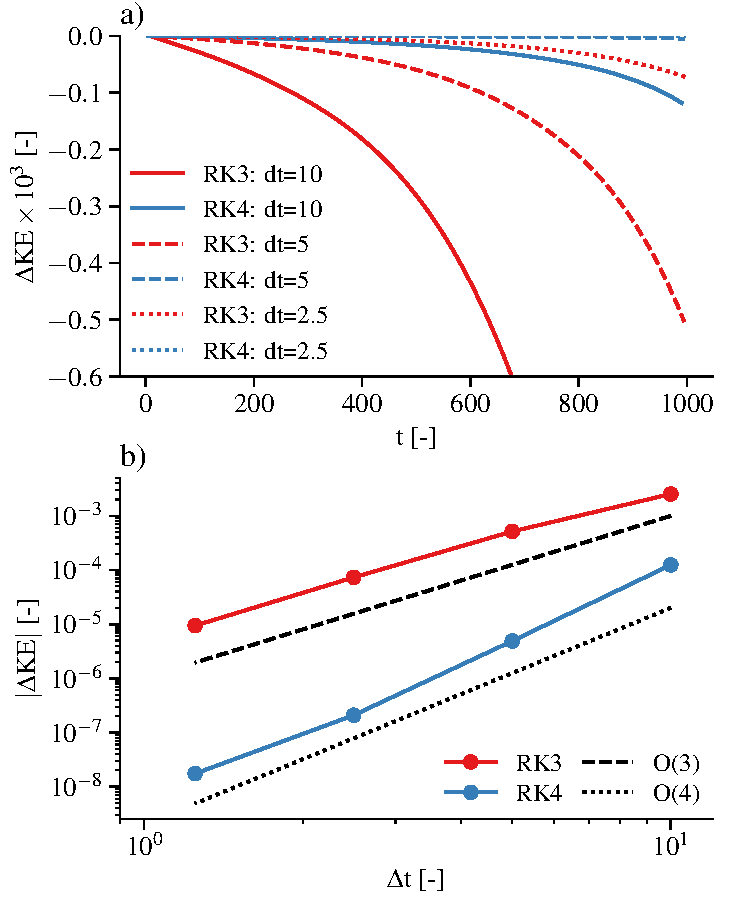
\includegraphics[width=8.3cm]{figs/timeconvergence.pdf}
\end{center}
\caption{Time evolution of the energy loss during 1000 time units of random noise advection for the RK3 and RK4 time integration schemes for three different time steps (a), and error convergence of the temporal discretization for the RK3 and RK4 scheme (b).}
\end{figure}

\subsection{Comparison against known case studies}
\subsubsection{Channel flow}

\begin{figure}[t]
\vspace*{2mm}
\begin{center}
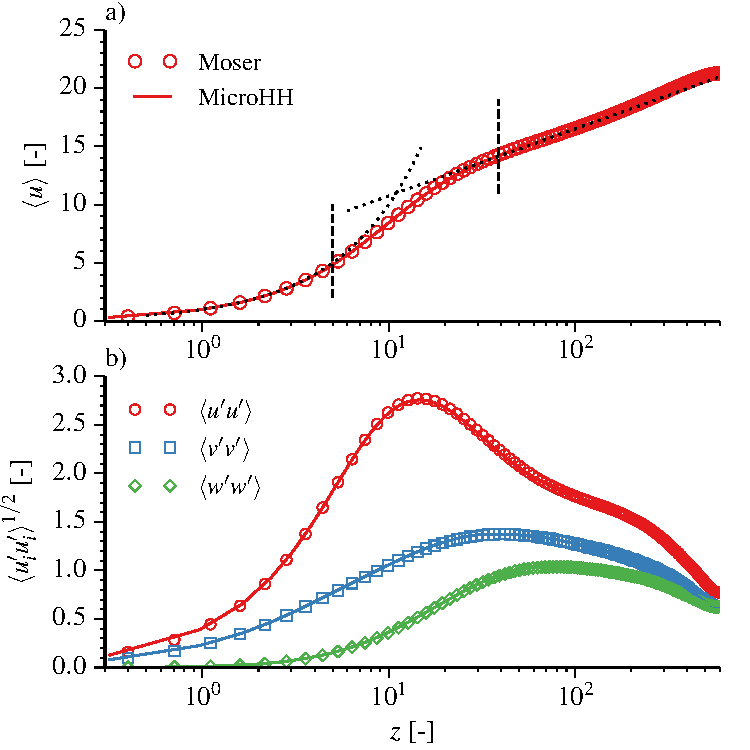
\includegraphics[width=8.3cm]{figs/gmd_m590_umean_var.pdf}
\end{center}
\caption{Moser590. Dashed line = spectra location. $z$ normalized with $u_\tau / \nu$, velocities with $u_\tau^{-1}$.}
\end{figure}

%% TWO-COLUMN FIGURES
\begin{figure*}[t]
\vspace*{2mm}
\begin{center}
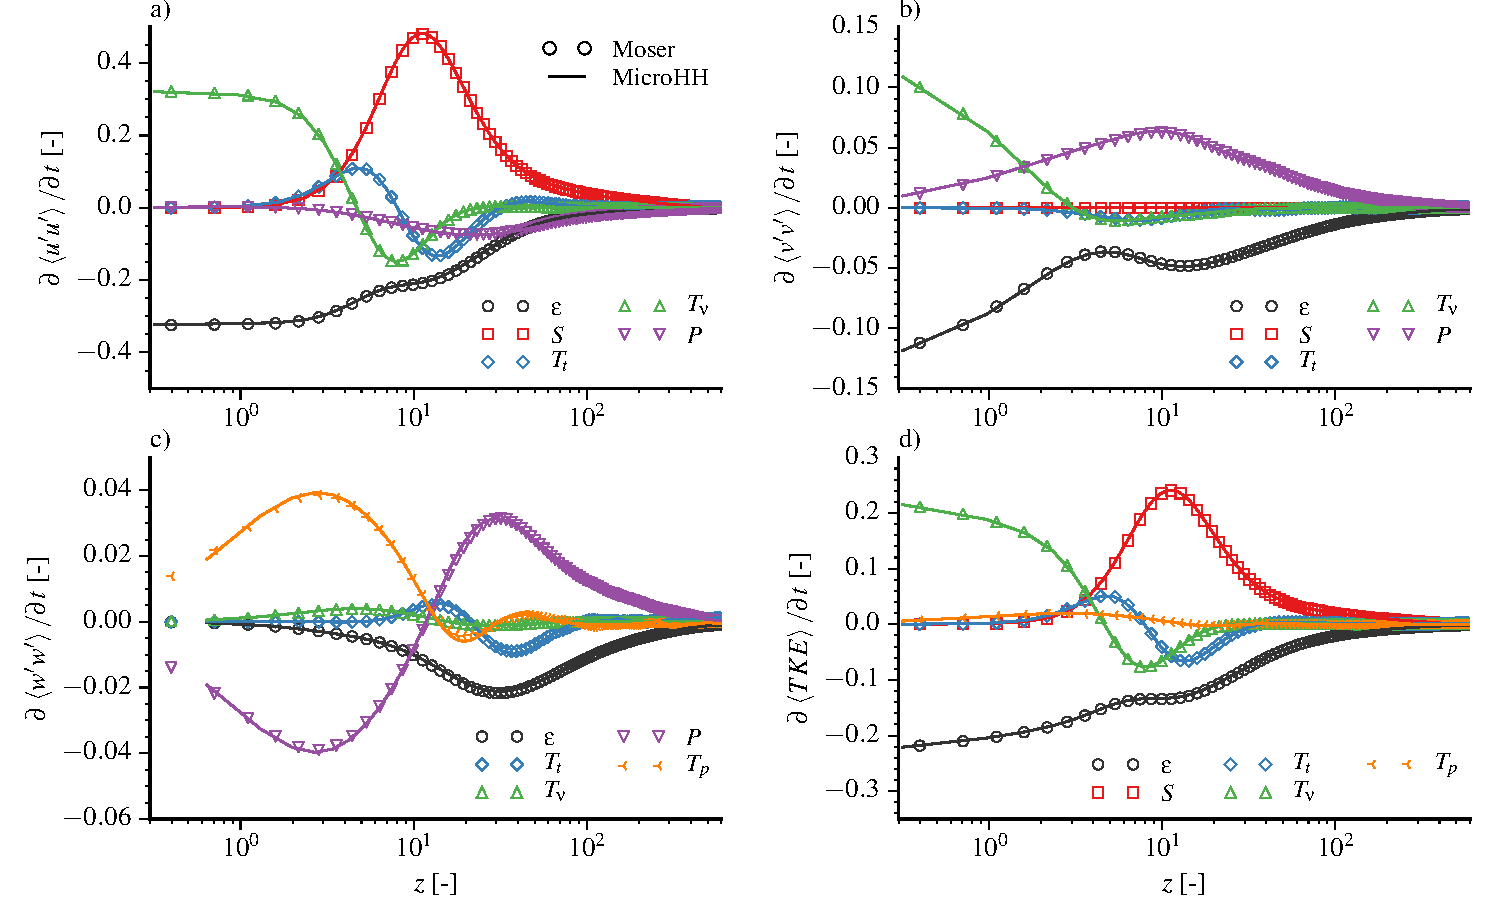
\includegraphics[width=16.6cm]{figs/gmd_m590_turb_budg.pdf}
\end{center}
\caption{Moser590 variance and TKE budgets. $z$ normalized with $u_\tau / \nu$, variances and TKE budget with $\nu / u_\tau^{4}$.}
\end{figure*}

%% TWO-COLUMN FIGURES
\begin{figure*}[t]
\vspace*{2mm}
\begin{center}
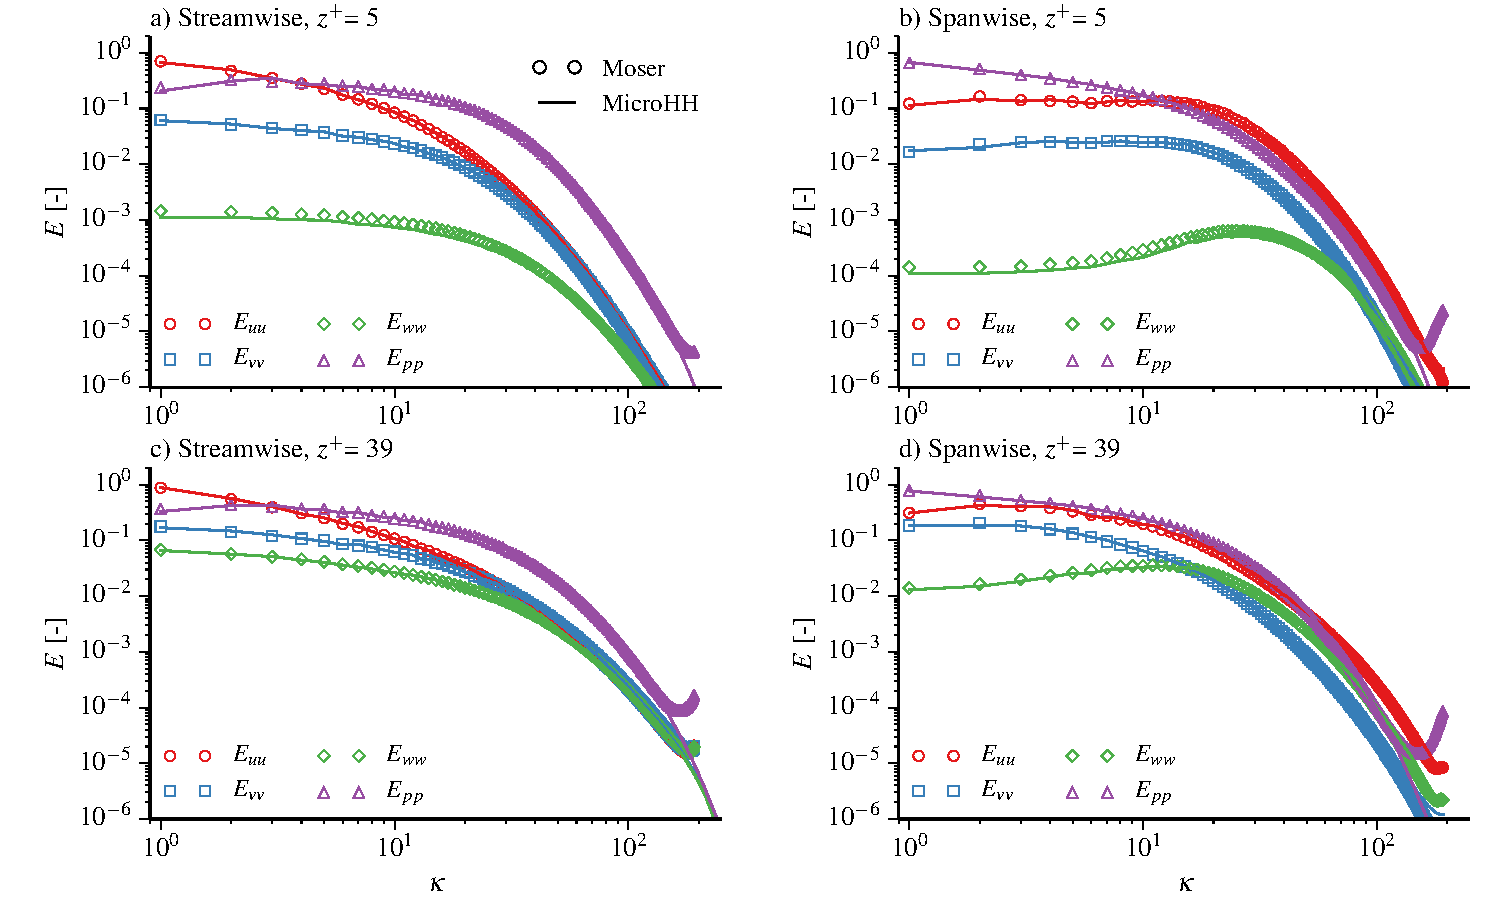
\includegraphics[width=16.6cm]{figs/gmd_m590_spectra.pdf}
\end{center}
\caption{Moser590 spectra, velocity spectra are normalized with $u_\tau^{-2}$, pressure spectra with $u_\tau^{-4}$}
\end{figure*}

\subsubsection{Dry CBL}
\subsubsection{Bomex}
\subsubsection{ARM}
\subsubsection{GABLS1}

\begin{figure*}[t]
\vspace*{2mm}
\begin{center}
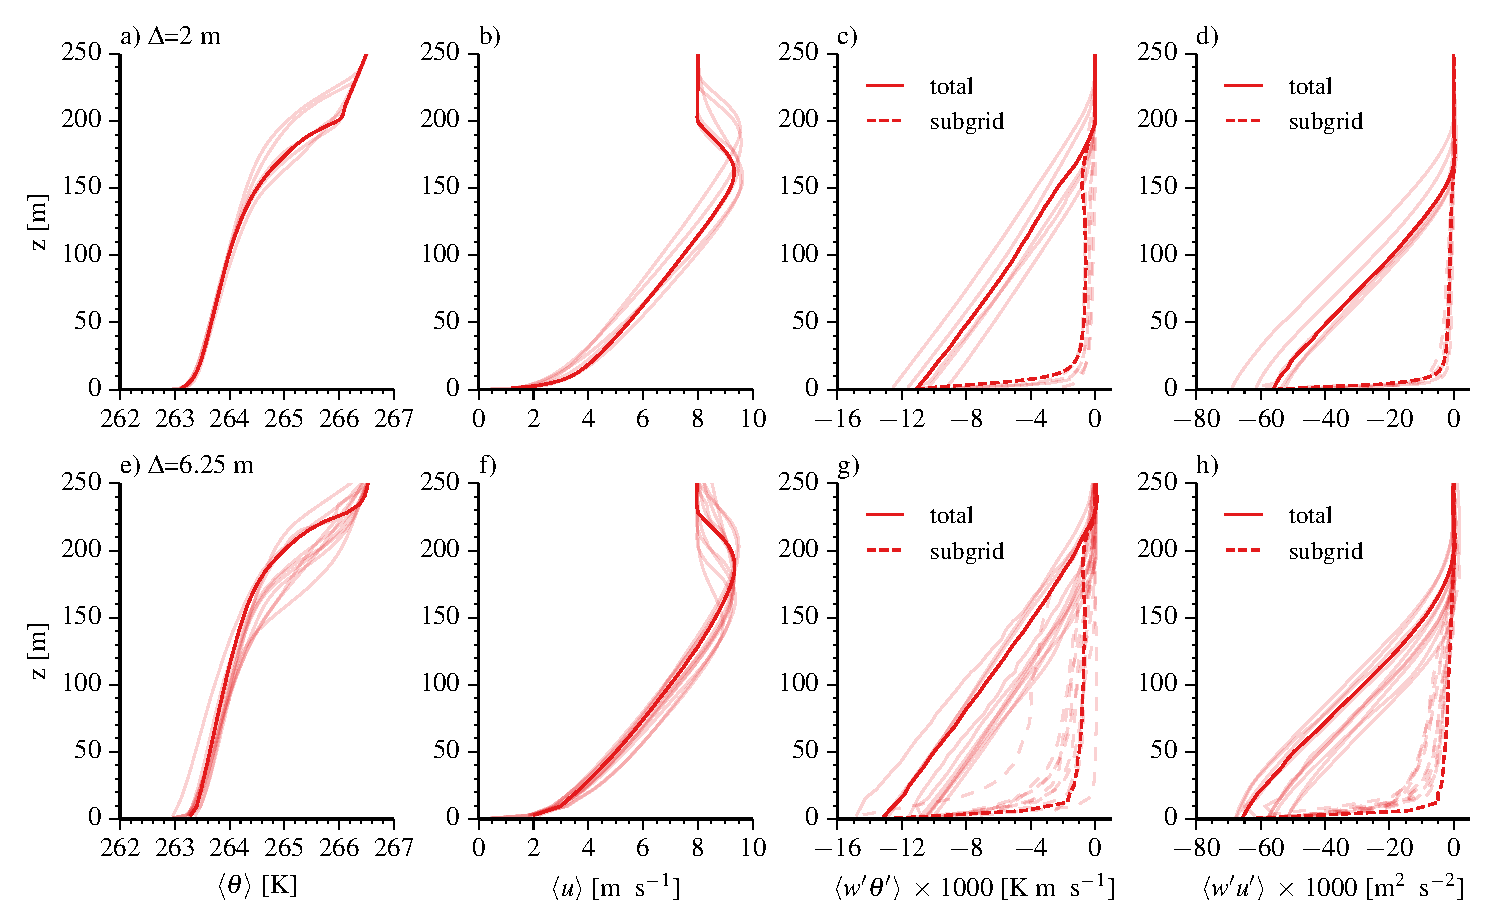
\includegraphics[width=16.6cm]{figs/gmd_gabls_mean_prof.pdf}
\end{center}
\caption{GABLS1 profiles}
\end{figure*}

\begin{figure}[t]
\vspace*{2mm}
\begin{center}
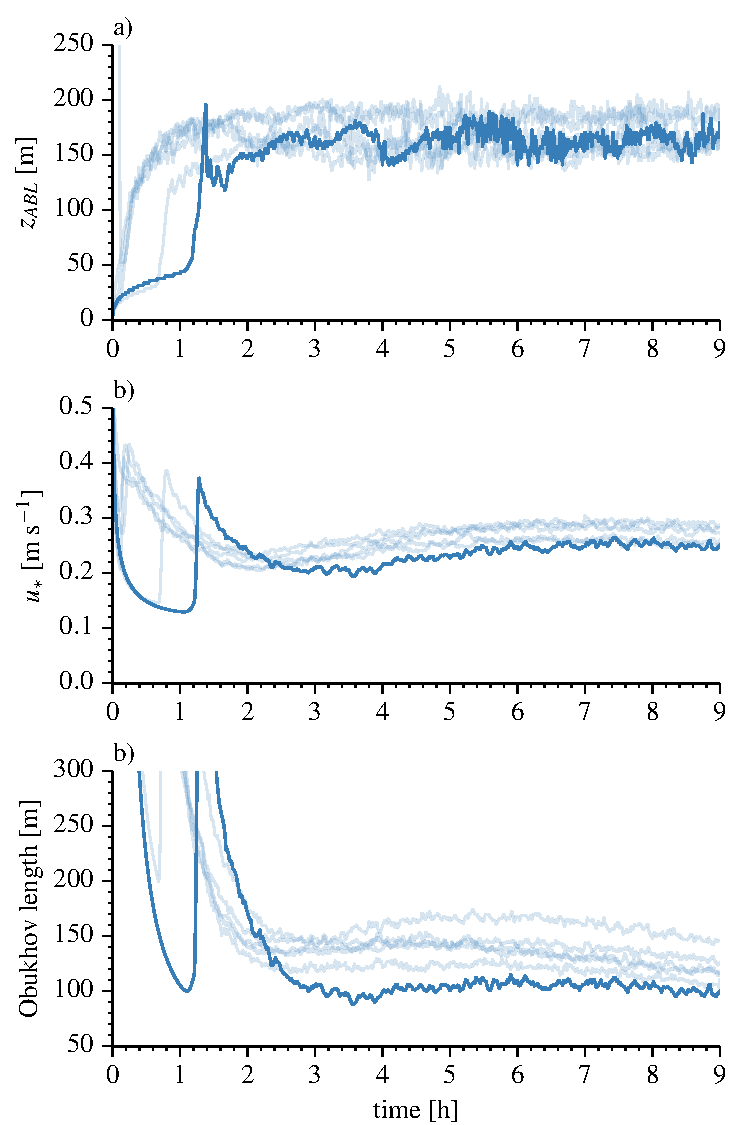
\includegraphics[width=8.3cm]{figs/gmd_gabls_tser.pdf}
\end{center}
\caption{GABLS1 time series}
\end{figure}

\subsubsection{Slope flow}

\conclusions  %% \conclusions[modified heading if necessary]

\bibliographystyle{copernicus}
\bibliography{../../misc/refs}

\end{document}
